\subsection{Aplicação Painel - segunda via código de barras}
\subsubsection*{Descrição do caso de uso}
Caso pretenda, um utilizador do painel também pode re-imprimir um código de barras sem necessidade de abrir a aplicação Fábrica. Para isso o utilizador necessita pressionar o botão\textit{ segunda via} da linha referente ao registo que pretende atualizar. Pelo facto de ser apenas uma procedimento executado em \textit{background}, não possui nenhuma \textit{view}.

\subsubsection*{\textit{Models} compatíveis com o caso de uso}
Este caso de uso é compatível com os \textit{models} Recolhas, Produto Acabado.

\subsubsection*{Fluxo do caso de utilização}
O caso de uso inicia-se quando o utilizador pressionar o botão 2ª via de código de barras da linha do registo. Um novo separador abre-se com o código de barras pronto a ser impresso, tal como demonstrado na figura \ref{fig:sd_2_via_painel}.


\begin{figure}[H] 
	\begin{center}
		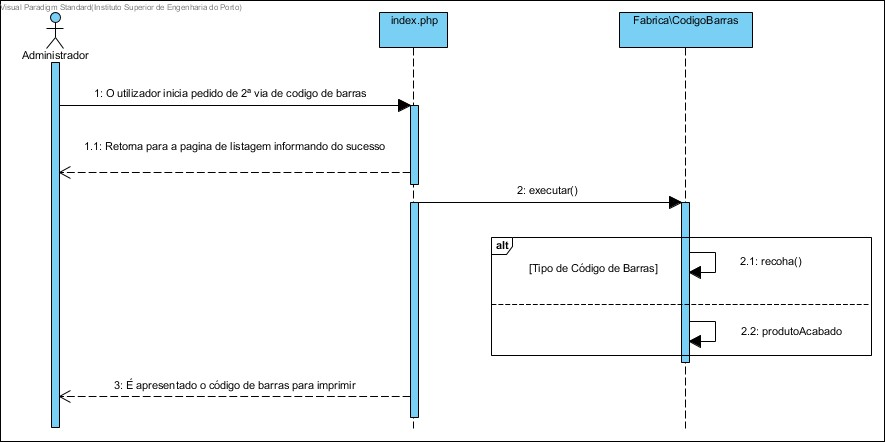
\includegraphics[width=\textwidth,keepaspectratio]{figuras/Diagramas_vp/SD_Painel_6_2_via_Codigo_de_Barras.jpg}
		\caption{Diagrama de sequência imprimir 2ª via do código de barras}
		\label{fig:sd_2_via_painel} 
	\end{center}
\end{figure}